\documentclass[tikz, border=16pt]{standalone}
\usepackage{tikz}
\usetikzlibrary{arrows.meta, positioning, calc, backgrounds}
\usepackage{amsmath}
\usepackage{lmodern}
\usepackage[T1]{fontenc}

%% ─── Node styles ─────────────────────────────────────────────────────────────
\tikzset{
  block/.style  = {draw, rectangle, thick,
                   minimum width=2.8cm, minimum height=1.35cm,
                   align=center, font=\small},
  sblock/.style = {draw, rectangle, thick,
                   minimum width=1.5cm,  minimum height=1.35cm,
                   align=center, font=\small},
  sum/.style    = {draw, circle, thick,
                   minimum size=0.82cm, inner sep=0pt},
  >=Stealth, thick
}

%% ─── Crosshair helper ────────────────────────────────────────────────────────
\newcommand{\crosshair}[1]{%
  \draw (#1) ++(0,  0.28cm) -- ++(0, -0.56cm);
  \draw (#1) ++(-0.28cm, 0) -- ++(0.56cm, 0);
}

\begin{document}
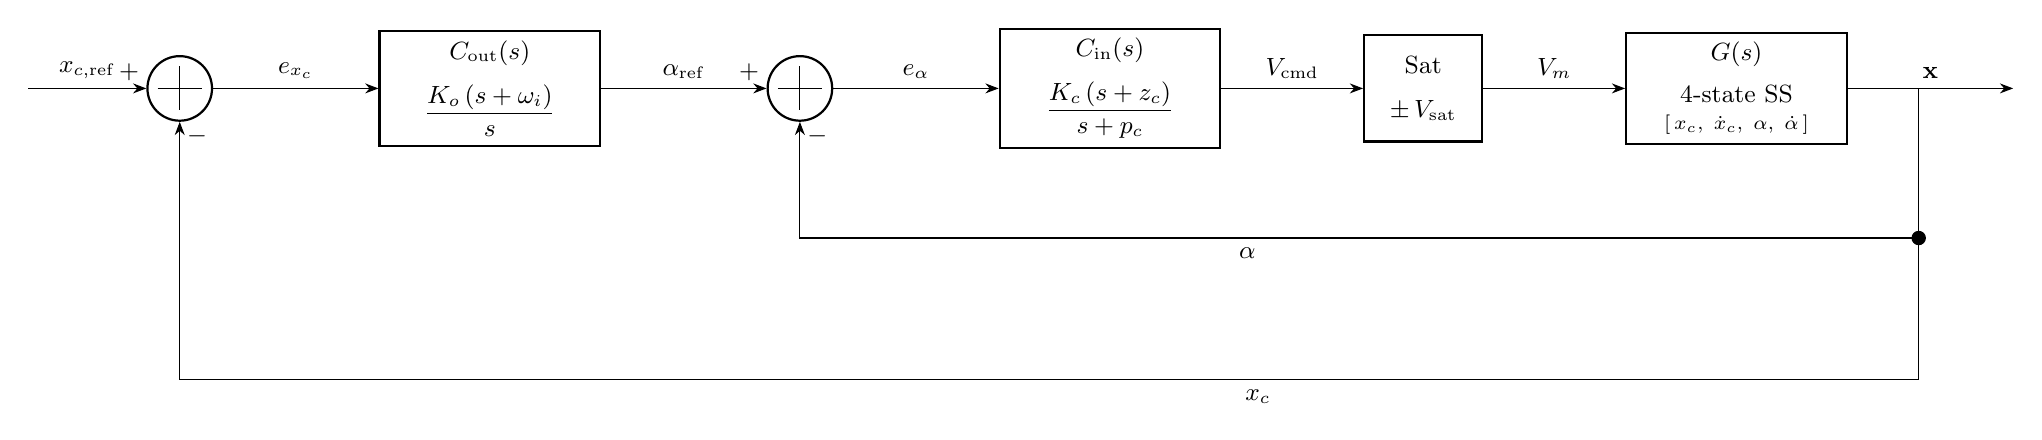
\begin{tikzpicture}

  %%──────────────────────────────────────────────────────────────────────────
  %%  FORWARD-PATH NODES
  %%──────────────────────────────────────────────────────────────────────────
  \node[coordinate]                     (r)   {};
  \node[sum,    right=1.5cm  of r]      (So)  {};
  \node[block,  right=2.1cm  of So]     (Co)
        {$C_{\mathrm{out}}(s)$\\[6pt]
         $\dfrac{K_o\,(s+\omega_i)}{s}$};
  \node[sum,    right=2.1cm  of Co]     (Si)  {};
  \node[block,  right=2.1cm  of Si]     (Ci)
        {$C_{\mathrm{in}}(s)$\\[6pt]
         $\dfrac{K_c\,(s+z_c)}{s+p_c}$};
  \node[sblock, right=1.8cm  of Ci]     (Sat)
        {Sat\\[5pt]$\pm\,V_{\mathrm{sat}}$};
  \node[block,  right=1.8cm  of Sat]    (G)
        {$G(s)$\\[4pt]
         \small 4-state SS\\[-1pt]
         \scriptsize$[\,x_c,\;\dot{x}_c,\;\alpha,\;\dot{\alpha}\,]$};
  \node[coordinate, right=2.1cm of G]  (y)   {};

  %%──────────────────────────────────────────────────────────────────────────
  %%  CROSSHAIRS ON SUMMING JUNCTIONS
  %%──────────────────────────────────────────────────────────────────────────
  \crosshair{So}
  \crosshair{Si}

  %%──────────────────────────────────────────────────────────────────────────
  %%  FORWARD-PATH WIRES
  %%──────────────────────────────────────────────────────────────────────────
  \draw[->] (r)   -- node[above]{\small$x_{c,\mathrm{ref}}$}     (So);
  \draw[->] (So)  -- node[above]{\small$e_{x_c}$}                 (Co);
  \draw[->] (Co)  -- node[above]{\small$\alpha_{\mathrm{ref}}$}   (Si);
  \draw[->] (Si)  -- node[above]{\small$e_{\alpha}$}              (Ci);
  \draw[->] (Ci)  -- node[above]{\small$V_{\mathrm{cmd}}$}        (Sat);
  \draw[->] (Sat) -- node[above]{\small$V_m$}                     (G);
  \draw[->] (G)   -- node[above]{\small$\mathbf{x}$}              (y);

  %%──────────────────────────────────────────────────────────────────────────
  %%  +/− LABELS  (outside the circle, adjacent to each port)
  %%──────────────────────────────────────────────────────────────────────────
  %% Convention: + on the horizontal input (west),  − on the feedback (south)
  \node[font=\small] at ($(So.west) +(-0.22cm, +0.21cm)$) {$+$};
  \node[font=\small] at ($(So.south)+(+0.22cm, -0.19cm)$) {$-$};
  \node[font=\small] at ($(Si.west) +(-0.22cm, +0.21cm)$) {$+$};
  \node[font=\small] at ($(Si.south)+(+0.22cm, -0.19cm)$) {$-$};

  %%──────────────────────────────────────────────────────────────────────────
  %%  FEEDBACK TRUNK
  %%──────────────────────────────────────────────────────────────────────────
  \coordinate (tap)  at ($(G.east)+(0.90cm, 0.00cm)$);
  \coordinate (fbA)  at ($(G.east)+(0.90cm,-1.90cm)$);  %% alpha branch-off
  \coordinate (fbX)  at ($(G.east)+(0.90cm,-3.70cm)$);  %% x_c   branch-off

  \draw (G.east) -- (tap);
  \draw (tap)    -- (fbX);

  %% Junction dot at alpha branch
  \filldraw[black] (fbA) circle (2.4pt);

  %% alpha → Si
  \draw[->] (fbA) -| node[pos=0.30, below]{\small$\alpha$}  (Si.south);

  %% x_c → So
  \draw[->] (fbX) -| node[pos=0.19, below]{\small$x_c$}     (So.south);

  %%──────────────────────────────────────────────────────────────────────────
  %%  LOOP BOUNDARY BOXES
  %%  Use let-\p inside \draw (valid) and \path (valid).
  %%  Never use let-\p directly inside \node[...] at ... (invalid).
  %%──────────────────────────────────────────────────────────────────────────
  \begin{scope}[on background layer]
    % Loop boundary boxes removed to avoid visual interference with signal lines
  \end{scope}

\end{tikzpicture}
\end{document}
